\chapter[A Arquitetura Implementada]{A Arquitetura Implementada}

Este capítulo apresenta detalhes sobre a execução do trabalho de conclusão de curso, detalhes da implementação realizada acerca da arquitetura bem como o protocolo de comunicação dentro desta.

A implementação realizada consiste de uma arquitetura de software baseada no modelo arquitetural SOA (orientado a serviços) responsável por promover a interação entre aplicações de \textit{software} desenvolvidas no contexto do grupo de orientação e trabalhos desenvolvidos em laboratórios de pesquisa e práticas de desenvolvimento de software na Universidade de Brasília. O protocolo de comunicação entre as aplicações também foi estabelecida por esta proposta.

Este capítulo está organizado em quatro seções principais. A seção 3.1 apresenta uma introdução, expondo fatos e necessidades que deram suporte à solução arquitetural proposta e implementada. A seção 3.2 trata do ambiente virtual criado com base na solução. A proposta arquitetural está detalhada na seção 3.3. Nesta última seção, também está descrito o protocolo utilizado, estabelecendo o formato de mensagem padronizado na arquitetura.

\section{Introdução}
Avanços tecnológicos, a criação de linguagens de programação, diferentes técnicas e paradigmas e outros conceitos relacionados ao desenvolvimento de software contribuem para que a necessidade de interação entre estes elementos seja emergente. Isto viabiliza a construção de sistemas cada vez mais robustos e inteligentes. Esta interação entre elementos de software não consistem de aplicações robustas que executam todas as suas atividades de forma independente de outras aplicações. Os sistemas de software mais modernos são desenvolvidos tomando como base outros paradigmas ou escritos em outras linguagens de programação e utilizando-se diferentes técnicas.

A fim de suprir esta necessidade de interação entre os diversos sistemas, foi criado um modelo arquitetural conhecido como Arquitetura Baseada em Serviços (ou \textit{Service-Oriented Architecture} - SOA) \cite{linthicum_soainrealworld_2007}. Este modelo arquitetural utiliza o conceito de serviço como uma unidade que representa uma funcionalidade reusável do sistema \cite{lewis_getting_2010}, além de trazer consigo como conceitos chave interoperabilidade, flexibilidade, extensibilidade e baixo acoplamento entre os diversos sistemas ou serviços \cite{josuttis_soa_2007}.

Para este trabalho de conclusão de curso, foi desenvolvida uma arquitetura baseada no modelo SOA para um ambiente heterogêneo com características predominante web (um ambiente virtual), propiciando que diversas aplicações desenvolvidas que se encontram armazenadas em repositórios não mais mantidos ou visitados sejam integradas como módulos da plataforma. Por meio do uso do modelo arquitetural proposto, foi possível integrar tais aplicações, ou serviços, de modo que estas trocam dados e fazem uso do serviço disponibilizado por outras, indepentemente das tecnologias utilizadas para o desenvolvimento das mesmas.

Um protocolo de comunicação entre as aplicações foi estabelecido, bem como o padrão de comunicação utilizado, uma vez que as aplicações produzidas por terceiros podem se comunicar de modo a se tornarem mais robustas e completas enquanto ferramentas.

Desta forma, foi possível prototipar uma plataforma virtual que contém resultados de trabalhos realizados por um grupo de orientandos de TCC e atividades desenvolvidos em laboratórios de pesquisa e práticas de desenvolvimento de software na Universidade de Brasília.

\section{O Ambiente Virtual}

Trabalhos realizados durante a execução de TCCs e em atividades e treinamentos desenvolvidos no âmbito de laboratórios de pesquisa e práticas de desenvolvimento de software no Campus Gama da Universidade de Brasília resultam, muitas vezes, em aplicações de software isoladas. Estas aplicações são armazenadas em repositórios pessoais de orientandos de TCCs ou do laboratório, e acabam por não serem divulgadas, incrementadas e mantidas por quem as criou.

Como exemplos de trabalhos realizados que resultaram em aplicações de interesse público, mas que não estão em uso ou manutenção, podem ser citados dois: um faz uma análise de aderência de perfis profissionais com base no currículo Lattes \cite{jesus_algoritmo_2014} e o outro faz a apresentação de resultados relevantes ao usuário de acordo com o perfil individual e de grupo de determinado usuário de uma plataforma virtual \cite{carvalho_sistema_2014}.

O ambiente virtual protipado neste projeto de TCC consiste no resultado da integração de aplicações já existentes.

\begin{figure}[!hbt]
\centering
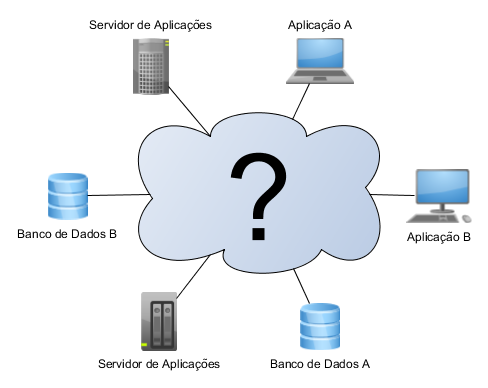
\includegraphics[scale=0.7]{figuras/ambiente_virtual.png}
\caption{Representação de um ambiente composto por aplicações integradas.}
\label{ambiente_virtual}
\end{figure}

A figura \ref{ambiente_virtual} apresenta a ideia do que é o ambiente virtual construído. Aplicações existentes que hoje se encontravam em repositórios aleatórios foram integradas com base na arquitetura proposta neste projeto de TCC. A interação entre tais elementos foi possível através do uso de mensagens padronizadas pelo protocolo estabelecido.

\section{A Arquitetura}

Esta seção apresenta os detalhes da arquitetura proposta e implementada baseada no modelo SOA, os aspectos deste modelo que foram adotados, e a forma como se relacionam.

As subseções apresentam os requisitos identificados, a arquitetura e detalhes sobre o protocolo de comunicação.

\subsection{Requisitos}
A partir da necessidade identificada de disponibilizar aplicações que foram desenvolvidas, bem como aquelas que estão em desenvolvimento e que serão desenvolvidas, através da plataforma virtual, algumas das principais características arquiteturais deste ambiente que influenciaram na escolha do modelo arquitetural para a construção da plataforma foram:

\begin{itemize}
\item A comunicação entre as aplicações deve permitir a troca de dados independentemente das tecnologias utilizadas para seu desenvolvimento.
\item O acoplamento entre aplicações deve ser o mínimo possível.
\item Extensibilidade, permitindo que novas aplicações/componentes sejam inseridas à plataforma.
\item Escalabilidade, fornecendo suporte para que diversas aplicações (ou componentes) sejam aderidas à plataforma.
\item Flexibilidade,  possibilitando a extensão da plataform sem que a arquitetura original seja modificada drasticamente.
\end{itemize}

A partir destas características, foi implementado o uso do modelo arquitetural SOA. Desta forma, a plataforma virtual tem conhecimento sobre as aplicações por meio das interfaces disponibilizadas, mas não precisa ter conhecimento sobre como ou quais tecnologias foram utilizadas para o desenvolvimento das aplicações. As aplicações, neste contexto, também podem ser denominadas serviços ou funcionalidades da plataforma virtual.

\subsection{A arquitetura escolhida}

A proposta de arquitetura implementada faz uso da abordagem de implementação de SOA chamada "\textit{Hub-and-spoke}", onde a interface de comunicação entre os serviços é única e pode ser realizada com o uso de um barrameneto de serviços ou um Enterprise Service Bus (ESB) \cite{Bianco2007}.

O barramento de serviços é um recurso utilizado na implementação da arquitetura baseada no modelo SOA para facilitar a troca entre mensagens entre as aplicações - ou serviços. Este barramento é uma ferramenta que implementa funcionalidades que roteiam as mensagens entre os usuários e provedores de um determinado serviço, transformam as mensagens e os dados para o formato aceito pelas aplicações e com protocolos múltiplos de comunicação através de adaptadores. Na arquitetura proposta, o protocolo de comunicação foi padronizado e a funcionalidade de roteamento de mensagens entre os serviços foi a mais explorada.

Sendo interoperabilidade um dos requisitos relevantes para a escolha do modelo arquitetural, o barramento de serviços foi visto como um recurso utilizado para ajudar a promover a interoperabilidade na arquitetura definida e na validação de políticas e critérios de segurança a serem definidas em trabalhos posteriores.

\begin{figure}[!hbt]
\centering
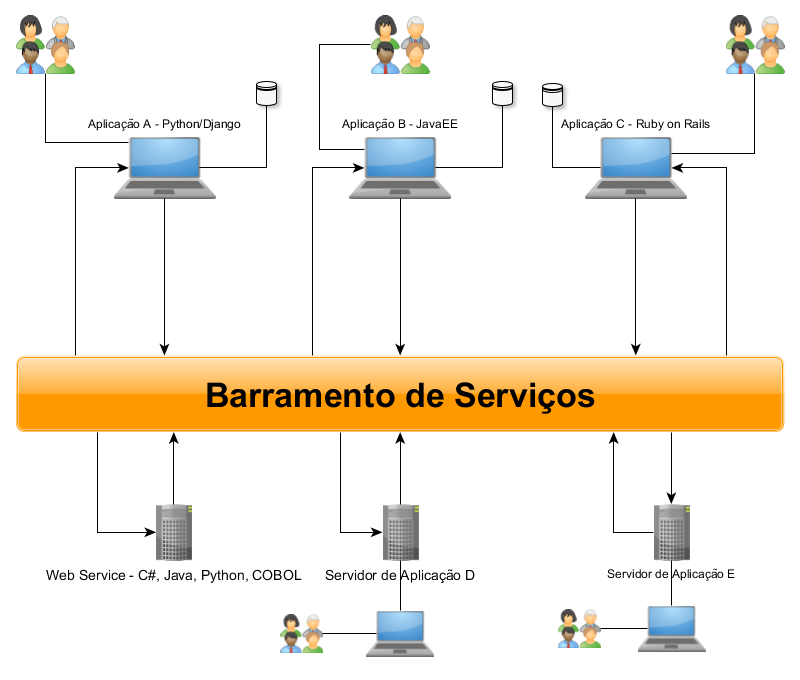
\includegraphics[scale=0.4]{figuras/barramento_interoperabilidade.png}
\caption{Interoperabilidade em uma arquitetura baseada no modelo SOA.}
\label{barramento_interoperabilidade}
\end{figure}

A figura \ref{barramento_interoperabilidade} apresenta a interoperabilidade em uma arquitetura baseada no modelo SOA:  as diversas aplicações fazem a requisição dos serviços disponíveis por meio do uso do barramento de serviços, que também pode ser interpretado como um barramento de aplicações. As aplicações podem ser desenvolvidas utilizando-se tecnologias e paradigmas distintos. A troca de dados entre elas são de forma bidirecional via mensagens de requisição e de resposta entre as aplicações usuário (requisitam operações dos serviços) e os serviços (processam as requisições e fornecem a resposta correspondente).

Um fato interessante na arquitetura implementada (figura \ref{barramento_interoperabilidade}): as aplicações podem operar tanto em modo \textit{standalone}, sendo executadas de forma independente dos outros serviços ou aplicações, quanto como um serviço para a plataforma virtual ou para outras aplicações que tenham conhecimento da existência e do protocolo em uso por este serviço.

O ESB é uma ferramenta que fornece as funcionalidades de um barramento de serviços. Seu uso garante que as requisições realizadas sempre terão uma resposta, mesmo sendo algo que indique a inatividade do serviço requerido ou a não autorização para acesso à operação requisitada. Ao se adicionar um novo serviço à arquitetura utilizando o ESB, os procedimentos a serem seguidos pelo barramento são especificados. Estes procedimentos dizem respeito ao processamento e encaminhamento das mensagens tanto de requisições quanto das respostas recebidas.

Com base nos requisitos essenciais levantados e no estudo realizado sobre o modelo arquitetural SOA, o modelo proposto implementado pode ser visto na figura \ref{uso_esb}.

\begin{figure}[!hbt]
\centering
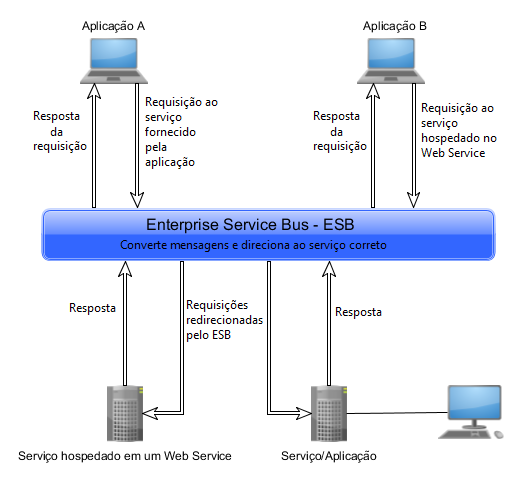
\includegraphics[width=0.7\textwidth]{figuras/uso_esb.png}
\caption{Proposta da arquitetura baseada no modelo SOA com o uso de um ESB.}
\label{uso_esb}
\end{figure}

A comunicação entre aplicações e serviços seguem o padrão de protocolo definido durante o desenvolvimento deste trabalho de conclusão de curso, para que seja mantida uma regra de execução na troca de informações. O protocolo também facilitará a adição de um novo serviço à arquitetura no que diz respeito aos procedimentos de transformação dos dados e adaptação entre tecnologias e protocolos de transporte e comunicação adotados.

\subsubsection{Ferramenta ESB}
Existem algumas ferramentas tipo ESB disponíveis e em uso por grandes organizações, tais como JBoss ESB\footnote{Para acesso a mais informações: http://jbossesb.jboss.org/}, Mule ESB\footnote{Mais informações em: https://www.mulesoft.com/platform/soa/mule-esb-open-source-esb}, Zato\footnote{\textit{Link} para acesso a mais informações: https://zato.io/docs/index.html}, WSO2 ESB\footnote{Informações podem ser encontradas em: http://wso2.com/products/enterprise-service-bus/} e ErlangMS\footnote{\textit{Link} para repositório com mais informações: https://github.com/erlangMS/msbus}. Para o conhecimento sobre a viabilidade de execução do trabalho aqui proposto, algumas destas ferramentas foram levantadas, e, sendo o ESB um elemento importante para a implementação deste TCC, uma análise destas ferramentas foi realizada. Os critérios utilizados para a seleção foram:

\begin{itemize}
\item Ser uma ferramenta de código aberto e/ou \textit{free};
\item Possuir documentação e tutoriais disponíveis;
\item Facilidade para implantação e instalação;
\item Facilidade para uso;
\item Possibilidade de de uso de conectores (customizados e existentes);
\item Suporte ao formato de mensagem escolhido para a implementação do protocolo (REST e JSON);
\item Permitir a conexão de serviços ao barramento independentemente da linguagem ou paradigma de programação.
\item Suporte ao ambiente operacional Linux.
\end{itemize}

Outro aspecto importante que foi analisado diz respeito à licença de distribuição da ferramentas ESB. A licença de distribuição pode interferir no uso e propriedade da arquitetura distribuída estabelecida por este projeto.

O levantamento mostrou que as ferramentas que poderiam ser utilizadas para a implementação da arquitetura eram o JBoss ESB, WSO2 ESB e ErlangMS. Foram realizados testes e pesquisas sobre as ferramentas ESB com base nos critérios estabelecidos. O resultado desta análise é exibido na Tabela \ref{analise_ferramentas}.


\begin{table}[!h]
\centering
\caption{Análise de ferramentas ESB segundo critérios definidos.}
\label{analise_ferramentas}
\begin{tabular}{|p{7cm}|c|c|c|c|}
\hline
Critérios & \multicolumn{1}{l|}{WSO2 ESB} & \multicolumn{1}{l|}{JBoss ESB} & \multicolumn{1}{l|}{ErlangMS} \\ \hline
Código aberto e/ou \textit{free} & Sim & Sim & Sim \\ \hline
Documentação e tutoriais         & Sim & Sim & Sim \\ \hline
Facilidade para implantação e instalação     & Sim & Não & Sim \\ \hline
Facilidade para uso              & Sim & Sim & Sim \\ \hline
Uso de conectores                & Sim & Sim & Sim \\ \hline
Suporte a REST e JSON            & Sim & Sim & Sim \\ \hline
Conexão de serviços ao barramento independentemente da linguagem ou paradigma de programação & Sim & Não & Sim \\ \hline
Suporte a Linux SO               & Sim & Sim & Sim\\ \hline
Linceça de Distribuição          & Apache2 & GNU GPL & Não possui \\ \hline
\end{tabular}
\end{table}

A Tabela 1 apresenta um sumário da análise realizada. É possível verificar que os critérios relacionados a usabilidade, implantação e instalação não foram alcançados pelo JBoss ESB, mesmo existindo uma grande comunidade aderente ao uso desta ferramenta. Concluiu-se também que esta ferramenta é limitada ao uso de serviços escritos em Java, uma vez que não foram encontrados documentos ou tutoriais com exemplos claros da utilização do JBoss ESB para disponibilização de serviços desenvolvidos em outras linguagens  de programação. As ferramentas ErlangMS e WSO2 ESB apresentaram um resultado geral satisfatório de acordo com os critérios de seleção elicitados. O único produto ESB não licenciado é o ErlangMS.

Com relação a documentação e tutoriais, ErlangMS possui pouca documentação disponível quando comparada com as outras ferramentas. WSO2 ESB destacou-se com relação ao uso de conectores, uma vez que foi possível utilizar conectores já existentes e disponíveis na plataforma da própria WSO2\footnote{https://store.wso2.com/store/assets/esbconnector/list} , bem como a construção de novos conectores. Estes conectores são contruídos de forma independente de tecnologia, promovendo a interoperabilidade da arquitetura. JBoss ESB provê modelos para a construção de conectores, porém esta funcionalidade parece ser limitada ao contexto de aplicações Java. Embora ErlangMS tenha como objetivo promover a integração de serviços de maneira independente de tecnologias, atualmente existem conectores disponíveis apenas para aplicações Java. Além disto, a construção de conectores para aplicações em outras linguagens é uma atividade complexa e que  não faz parte do escopo deste projeto.

As pesquisas e testes realizados resultaram na escolha do WSO2 ESB como o componente ESB utilizado na implementação da arquitetura proposta. Uma documentação disponível e extensiva, além da colaboração de usuários por meio da divulgação de tutoriais, possibilitam a fácil instalação, implantação e uso da ferramenta. Além disto, conectores podem ser utilizados para disponibilização de serviços e APIs independentemente de tecnologias utilizadas para a construção do serviço. 

\subsection{Protocolo de comunicação}

No âmbito da proposta de uma arquitetura de software baseada no modelo SOA, é necessário que seja estabelecido um protocolo de comunicação. Este protocolo estabelece como as aplicações que oferecem e utilizam os serviços contidos na arquitetura irão se comunicar.

Após levantamento de modelos de protocolos, formatos e padrões de mensagens existentes optou-se pelo uso do modelo REST \cite{rozlog_restesoap_2013}. Este modelo de protocolo foi escolhido por ser de fácil uso, podendo ser implementado em diversas linguagens de programação (principalmente aquelas que são destinadas ao desenvolvimento de plataformas para a web) e em diversos sistemas operacionais. O modelo REST utiliza o HTTP como protocolo de transporte, contribuindo para que a comunicação entre diversas aplicações seja realizada de maneira mais estável.

A arquitetura do protocolo REST aceita diferentes formatos tais como: JSON, CSV e texto simples. O formato definido para uso no protocolo desta proposta de TCC é o JSON, por ser um formato que permite a composição da mensagem através de chaves e valores. Assim, quando de posse da mensagem, os valores podem ser extraídos de acordo com a chave. As informações de chave e valores retornados por uma dada operação de um serviço devem estar contidas na especificação da interface de um serviço.

%Alguns serviços podem necessitar de autenticação e autorização para acesso ao mesmo, porém outros estarão disponíveis para uso sem a necessidade de que tais recuros de segurança sejam implementados. Os requisitos de segurança na troca de dados deverão ser planejados em trabalhos futuros.

A fim de permitir o acesso ao serviço, as aplicações devem disponibilizar uma API REST para que os recursos sejam manipulados através das operações. Do inglês "\textit{Application Programming Interface}", uma API é um conjunto de operações e padrões de programação criadas por empresas de software a fim de disponibilizar seus serviços por meio de um aplicativo de software ou plataforma Web \cite{canaltech_o_2015}. O uso de uma API permite a construção de plataformas Web a partir do uso de funções de outras aplicações \cite{canaltech_o_2015}. Um exemplo é a API fornecida pelo Facebook, utilizada para realização de login utilizando credenciais da rede social, permitindo o acesso a fotos e conteúdo do perfil do usuário.

O fluxo básico do protocolo de comunicação entre os provedores e usuários dos serviços pode ser visto na figura \ref{fluxo_basico_protocolo}.

\begin{figure}[htb]
\centering
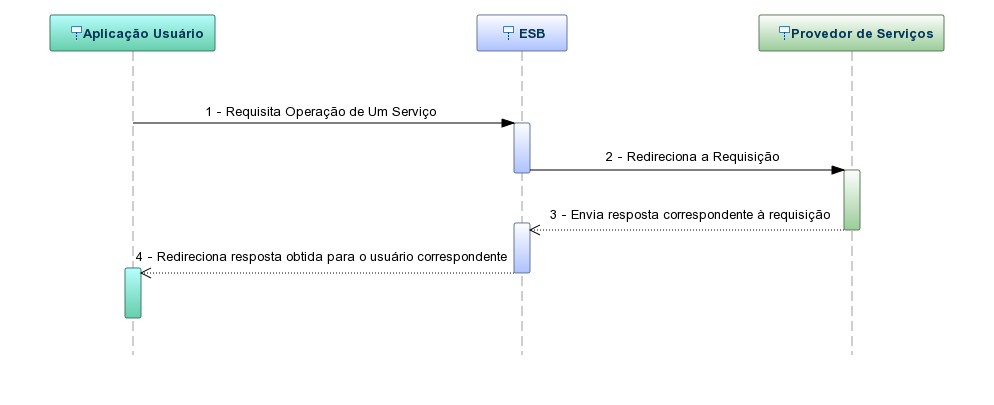
\includegraphics[width=1\textwidth]{figuras/fluxo_basico_protocolo.png}
\caption{Fluxo básico do protocolo de comunicação.}
\label{fluxo_basico_protocolo}
\end{figure}

Ao realizar a requisição à uma operação disponibilizada pelo serviço, a ferramenta ESB trata tal requisição e redireciona à aplicação provedora do serviço. A resposta correspondente também é intermediada pelo ESB e enviada para a aplicação usuária de serviços.

O ESB é o elemento que detêm o conhecimento sobre os serviços providos na plataforma. É o ator responsável por realizar a entrega das mensagens de requisição e de resposta dos serviços. Caso necessário, também tem a  responsabilidade de realizar a transformação/adaptação dos formatos das mensagens e dos protocolos usados.

\subsubsection{Formato das Mensagens}
O formato escolhido para a troca de mensagens entre as aplicações é o JSON. A escolha foi realizada pelo fato deste formato de mensagem ser leve, de fácil entendimento e implementação, além de permitir que não seja difícil a recuperação dos dados em qualquer linguagem de programação.

O formato JSON é baseado em um esquema de chave-valor, onde a chave identifica um atributo, um dado, e o valor é o dado em si, o valor quantitativo ou qualitativo do atributo indicado pela chave. Este formato de mensagem adotado, pode ser tratado na aplicação como uma mensagem JSON ou como uma cadeia de caracteres, a depender da linguagem de programação adotada na construção da plataforma virtual e dos serviços disponibilizados.

Assim, para realizar uma requisição, a aplicação que executa o papel de usuário de um serviço indica o serviço e a operação desejada, o formato da mensagem (JSON por padrão) e os valores necessários para que o serviço seja executado corretamente, indicados pela API disponibilizada pelo mesmo. Da mesma forma, a resposta também é gerada em formato JSON, porém, a aplicação que provê serviços, retorna apenas a resposta da mensagem no padrão chave-valor. A seguir, podem ser visualizados um exemplo de requisição e outro de reposta, ambos em formato JSON.

\definecolor{verde}{rgb}{0.25,0.5,0.35}
\definecolor{jpurple}{rgb}{0.5,0,0.35}

\lstset{
  language=Java,
  basicstyle=\ttfamily\small, 
  keywordstyle=\color{jpurple}\bfseries,
  stringstyle=\color{blue},
  commentstyle=\color{verde},
  extendedchars=true, 
  showspaces=false, 
  showstringspaces=false, 
  numbers=left,
  numberstyle=\tiny,
  breaklines=true, 
  backgroundcolor=\color{cyan!10}, 
  breakautoindent=true, 
  captionpos=b,
  xleftmargin=0pt,
  tabsize=4,
  texcl=true
}
\begin{lstlisting}
//Exemplo de uma mensagem de requisição de serviço em formato JSON de uma 
//aplicação usuário.

url = "http://localhost:8000/services/facebookConnector"
headers = {'Action':'urn:getUserDetails', 
	'Content-type':'application/json'}
payload = {'apiUrl':'https://graph.facebook.com', 
	'apiVersion':'v2.5',
	'accessToken':access_token,
	'fields':'id,,name,email,age_range,birthday'}

//Exemplo de uma mensagem de resposta de requisição em formato JSON.
{'id':'1', 'name':'user_name', 'email':'user@email.com', 
	'age_range':'20-25', 'birthday':'dd/mm/yyyy'}
\end{lstlisting}

O código exibe os valores necessários para realizar uma requisição ao serviço fornecido pela rede social Facebook através de sua API. Para a chamada do serviço, são necessários a especificação do endereço do serviço, indicado pela \textit{url}; \textit{headers} guarda os valores da operação a ser executada pelo serviço ('\textit{Action}') e o formato da mensagem ('\textit{Content-type}'); os valores necessários para a execução da operação requisitada estão contidos no \textit{payload} também em formato \textit{{'chave':'valor'}}.

A parte de código descrito mostra apenas exemplos do uso do formato de mensagem JSON para realizar uma requisição e de mensagem obtida como resposta advinda do serviço. Pode-se ver que os valores são correspondentes à uma chave conhecida por ambas as aplicações, permitindo que as aplicações (provedora e usuária de serviços) possam comunicar-se entre si de forma padronizada e conhecida por ambas as partes.

\section{Fechamento do Capítulo}
Neste capítulo, foi apresentada a ideia principal do projeto desenvolvido durante a realização do TCC. Foi elaborada uma arquitetura baseada no modelo SOA para a integração de aplicações resultantes de orientações de TCC e de atividades  desenvolvidas em laboratórios de pesquisa e práticas de desenvolvimento de software na Universidade de Brasília. Para tanto, aqui foram detalhadas as características que fizeram parte da solução proposta, com o uso de uma ferramenta do tipo ESB e um protocolo de comunicação padronizado, baseado no modelo REST.

A utilização de uma ferramenta que contenha as funcionalidades de um ESB (roteamento, transformação e formatação de dados) permite que a complexidade de implementação da arquitetura seja reduzida, uma vez que não há a necessidade de um serviço fornecer múltiplas interfaces. Isto colabora para que a interoperabilidade, flexibilidade e extensibilidade almejada tenha sido mais facilmente realizada.
